% !TeX spellcheck = en_US
\documentclass[
12pt,
a4paper, 
%oneside, % Uncomment this for digital
twoside  % Use twoside for printing.
openright % Uncomment this for printing
]{book}

% If you use twoside, it will leave different margin for left and right. 
% Initially you think it is unintutive but it is actually how book margins are left. 
% See this for further infomation -- https://tex.stackexchange.com/a/319146/105124

%\usepackage{showframe} % This is to check margin area, you dont need it in general

\usepackage[utf8x]{inputenc}

% Footnote related
\usepackage[bottom]{footmisc} %Footnotes in Tables. Load this before hyperref

\author{Rohit Suratekar}
\usepackage[pdftex,
pdfauthor={Rohit Suratekar},
pdftitle ={Understanding structure and dynamics of the Drosophila PI(4,5)P2 cycle with mathematical models.},
pdfsubject={Computational Cell Biology},
pdfkeywords={PIP2 Cycle, Mathematical Model, PIP2, Thesis}, hidelinks]{hyperref} %References and hyperlinks 
% Remove Hidelinks option from above if you want links

\usepackage{graphicx, float, tikz-cd, xcolor, subcaption, chemfig} %Figures and Graphics
\usepackage{caption, tabularx, multirow, threeparttable, float} %Tables related
\usepackage{amsmath, amsfonts, amssymb, mathtools, calc} %Maths and Equations
\usepackage{standalone} % load only in the main file
\usepackage{fancyhdr} %For header
\usepackage{emptypage} % Removes header from empty pages
\usepackage{longtable} % Multipage Tables
\usepackage{makeidx} %To make index page
\usepackage[totoc]{idxlayout} %To get index into TOC
\usepackage[acronym,toc]{glossaries} %Acronyms, TOC option will add it to TOC
\usepackage[titletoc,title]{appendix} %For Appendix


\usepackage[version=3]{mhchem} %Chemistry reactions

%Tikz-cd setup
\usetikzlibrary{decorations.text}
\usetikzlibrary{positioning}

% To order citation within multiple citations
\usepackage[sort]{natbib}  %Need for sectionbib
\usepackage[sectionbib]{chapterbib} %References on each chapter

\allowdisplaybreaks %Allows equations to break page
\usepackage[final]{pdfpages} %Include PDF page

% Need to remove section numbers of appendix from TOC
\usepackage{etoolbox}
\appto\appendix{\addtocontents{toc}{\protect\setcounter{tocdepth}{0}}}
% reinstate the correct level for list of tables and figures
\appto\listoffigures{\addtocontents{lof}{\protect\setcounter{tocdepth}{1}}}
\appto\listoftables{\addtocontents{lot}{\protect\setcounter{tocdepth}{1}}}


%Create new style to add header on each page
\pagestyle{fancy}
\renewcommand{\sectionmark}[1]{\markright{#1}}
\fancyhf{}
\makeatletter
\rhead{\fancyplain{}{\if@mainmatter \slshape\nouppercase{\leftmark}} \fi}
\makeatother
\lhead{\fancyplain{}{}} 
\cfoot{\fancyplain{}{\thepage}}

% Comment following Hypersetup during printing
\hypersetup{ 
	colorlinks   = true, %Colours links instead of ugly boxes
	urlcolor     = blue, %Colour for external hyperlinks
	linkcolor    = blue, %Colour of internal links
	citecolor   = red %Colour of citations
}

% Footnote related command
\newcommand\pubnote[1]{%
	\begingroup
	\renewcommand\thefootnote{}\footnote{#1}%
	\addtocounter{footnote}{-1}%
	\endgroup
}

\makeindex %Makes index file.
\makeglossaries %Make glossary file


\renewcommand*{\glstextformat}[1]{\textcolor{black}{#1}}
\renewcommand{\glsnamefont}[1]{\textbf{#1}}
\glssetwidest{consectetuer}

\newacronym{ea}{EA}{Example Acronyms}
\newacronym{yaa}{YAA}{Yet Another Acronyms}

 %Include add acronyms

% For generating random text. You don't need it 
\usepackage{blindtext}


% Following new definition to align table text to left in case of multi-row and multi-column
\usepackage{array}
\newcolumntype{L}[1]{>{\raggedright\let\newline\\\arraybackslash\hspace{0pt}}m{#1}}

% Appendix related. Remove appendix sections from appearning in table of content
\usepackage{etoolbox}
\appto\appendix{\addtocontents{toc}{\protect\setcounter{tocdepth}{0}}}
\appto\listoffigures{\addtocontents{lof}{\protect\setcounter{tocdepth}{1}}}
\appto\listoftables{\addtocontents{lot}{\protect\setcounter{tocdepth}{1}}}

\begin{document}
	\frontmatter
	\begin{titlepage}
	\centering
	\vfill
	{\huge\bfseries Understanding structure and dynamics of the \textit{Drosophila} PI(4,5)P\textsubscript{2} cycle using mathematical models \par}
	\vspace{2cm}
	{\Large A Thesis\par}
	\vfill
	Submitted to the\par
	{\Large Tata Institute of Fundamental Research, Mumbai\par
	for the degree of Doctor of Philosophy\par in Biology \par}
	\vspace{1cm}
	by\par
	\vspace{0.5cm}
	{\Large \bfseries Rohit Chandrakant Suratekar\par}
	\vfill
	
	% Bottom of the page
	{\large National Centre for Biological Sciences, Bangalore\par
		Tata Institute of Fundamental Research, Mumbai\par}
	{October, 2018}
\end{titlepage}
	\chapter[Declaration]{\centering Declaration}
This thesis is a presentation of my original research work. Wherever contributions of others are involved, every effort is made to indicate this clearly, with due reference to the literature, and acknowledgement of collaborative research and discussions. 
\\
The work was done under the guidance of Dr. Sandeep Krishna, at the Tata Institute of Fundamental Research, Mumbai.
\\\\\\\\
\null\hfill \textbf{ Rohit Suratekar}\\
\null\hfill National Centre for Biological Sciences-TIFR, Bangalore
\\\\\\\\
In my capacity as supervisor of the candidate’s thesis, I certify that the above statements are true to the best of my knowledge.
\\\\\\\\
\null\hfill \textbf{Dr. Sandeep Krishna}\\
\null\hfill  National Centre for Biological Sciences-TIFR, Bangalore\\
\\
\null\hfill \textbf{Date} : \qquad\qquad\qquad\qquad\qquad\\
	\chapter[Certificate]{\centering Certificate}
I certify that this thesis entitled “\textbf{Understanding structure and dynamics of the \textit{Drosophila} PI(4,5)P\textsubscript{2} cycle using mathematical models}” comprises research work carried out by \textbf{Rohit Chandrakant Suratekar} at National Centre for Biological Sciences under the supervision of \textbf{Dr. Sandeep Krishna} during the period 2012 - 2018 for the degree of Doctor of Philosophy of the Tata Institute of Fundamental Research (TIFR). The results presented in this thesis have not been submitted previously to this or any other University for a PhD or any other degree.
\\\\\\\\\\\\\\\\
\null\hfill \textbf{Head of Academics}\\
\null\hfill National Centre for Biological Sciences\\
\null\hfill Tata Institute of Fundamental Research\\
\null\hfill Bangalore\\
	\chapter[Publication]{\centering Publication}

\textbf{Suratekar Rohit}, Panda Aniruddha, Raghu Padinjat, Krishna Sandeep. Evidence of sinks and sources in the phospholipase C-activated PIP\textsubscript{2} cycle.\textit{ FEBS Lett}. 2018 Mar; 592(6):962-972. doi: \href{https://doi.org/10.1002/1873-3468.12998}{10.1002/1873-3468.12998}. Epub 2018 Feb 21. PubMed PMID: 29427502.
\\\\
{\footnotesize Content from the above publication has been incorporated in the thesis with permission from the publisher (License no: 4325120624150).}
	\chapter[Acknowledgments]{\centering Acknowledgments}

\Blindtext 

	% For this page we need to remove chapter title and space above the title

% Following definition will remove the chapter title
\makeatletter
\newcommand{\unchapter}[1]{%
	\begingroup
	\let\@makechapterhead\@gobble % make \@makechapterhead do nothing
	\chapter*{#1}  % Used * so that it won't appear in Table of Content
	\endgroup
}
\makeatother

%Adjust Vspace to shift chapter above so that without title it will look like middle of the space 
\unchapter{\vspace{-5cm}} 

% Make sure to use closed center enviornment instead \centering 
%else all other chapters will also become center
\begin{center}
	\topskip0pt
	\vspace*{\fill}
	{\large Dedicated to all \par}
	\vspace{0.5cm}
	{\LARGE whatever you want!}
	\vspace*{\fill}
\end{center}

% Following will remove the page number
\thispagestyle{empty}

	
	\printglossary[type=\acronymtype,title={Abbreviations}, style=alttree]
	\phantomsection
	\addcontentsline{toc}{chapter}{\listfigurename}
	\listoffigures
	\phantomsection
	\addcontentsline{toc}{chapter}{\listtablename}
	\listoftables
	\tableofcontents
	
	\mainmatter
	
\Blinddocument 
\index{example1}  Now example citation \cite{Suratekar2018} and new \gls{ea}. Now you can use acronym as \gls{ea} and it will show up in your acronym list. 

% After each chapter you can add biblography.
% If you want only one Biblography, remove following helper file and put content of it in main.tex
\clearpage
% This is helper file which you can use in every chapter if you want to have separate biblography for each chapter

% If you want only single biblography for all thesis, just copy paste following content at the end of main.tex

	\bibliographystyle{unsrt}
	\bibliography{main_ref}
	
	
\chapter{Second Example}

\section{Introduction}
\blindtext \index{example1}
\cite{Suratekar2018}. 

Second acronym will be \gls{yaa}. This also can be used further as \gls{yaa}. This is example of footnote\footnote{This is footnote.}.
\section{Figure Example}
\blindtext 
\begin{figure}
	\centering
	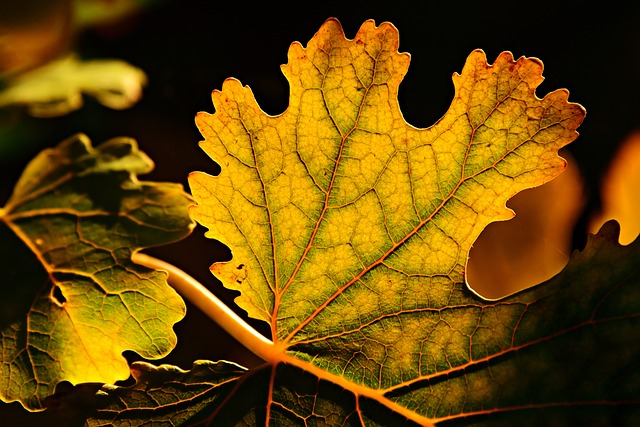
\includegraphics[width=0.7\linewidth]{figs/example}
	\caption{Figure downloaded from Pixabay.com and released under CC0.}
	\label{fig:example}
\end{figure}
\blindtext \index{example1}

\section{Table Example}
\blindtext \index{example2}

\begin{table}
	\centering
\begin{tabular}{|c|c|c|}
	\hline 
1	&  2& ssdfds \\ 
	\hline 
3	& 4 & sdfsdf \\ 
	\hline 
5	& 6 &  sdfsdf\\ 
	\hline 
7	&  8&  sdfsdfsdf\\ 
	\hline 
\end{tabular}
\caption{Example Table} 
\end{table}

\blindtext 

\blindtext 

% After each chapter you can add biblography.
% If you want only one Biblography, remove following helper file and put content of it in main.tex
\clearpage
% This is helper file which you can use in every chapter if you want to have separate biblography for each chapter

% If you want only single biblography for all thesis, just copy paste following content at the end of main.tex

	\bibliographystyle{unsrt}
	\bibliography{main_ref}
	
	
	
	% Switch off Caption
	\captionsetup{list=no}
	\begin{appendices}
\chapter{Extra Information}
\Blindtext 
\end{appendices}

	\printindex
\end{document}